\documentclass[11pt, a4paper]{article}

\usepackage{amsmath}
\usepackage{hyperref}
\usepackage{graphicx}
\usepackage{listings}
\usepackage{color}

\author{
  \textbf{KOTWAL ALANKAR SHASHIKANT}\\
  \texttt{12D070010}
  \and
  \textbf{ANAND KALVIT}\\
  \texttt{12D070032}
}
\title{Visual Odometry from Stereo Using Point-Set Matching}

\begin{document}
\maketitle
\newpage

\section{Introduction}
Odometry refers to the use of data from motion sensors to estimate change in position over time. One of the most reliable ways of estimation of 3-D structure using cameras is to use a calibrated stereo pair. Given the sequence of 3-D structures generated by the stereo camera, we can estimate the motion of the camera with respect to its environment as well as generate a 3-D map of the environment. This is usually referred to as visual SLAM (simultaneous localisation and mapping), which has wide applications in robotics and remote sensing. \\

\noindent We plan to implement a 6 DoF pose estimation algorithm using a calibrated stereo pair and generate a 3-D map of the environment simultaneously. We assume that scene illumination doesn't change much and most of the field of view of the camera is occupied by static parts of the environment. \\

\noindent In a nutshell, our job is to figure out what the translation and rotation of the camera is between two scenes as shown below. \\ \\ \\
\centerline{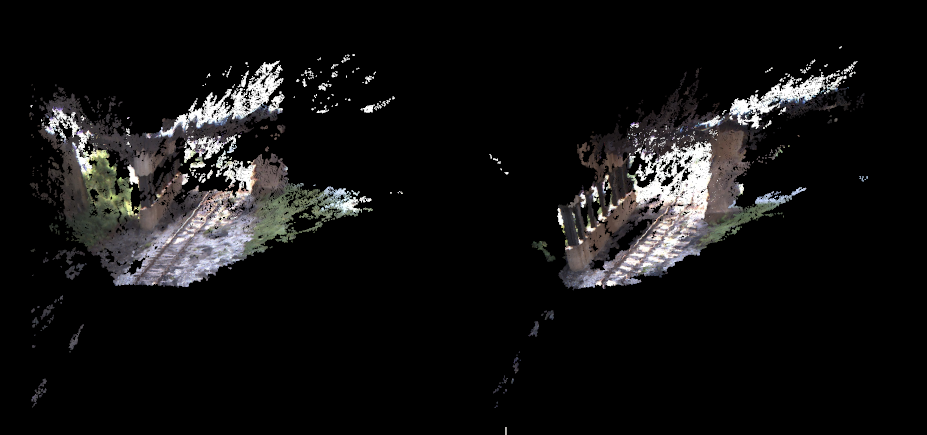
\includegraphics[scale=0.50]{pointclouds}}
\newpage

\section{Method}
We closely follow the method outlined in \cite{main}. The method involves modelling both the reference and the moving pointclouds as Mixture Models. We choose spherical Gaussian Mixtures and equal weights per-point for simplicity and easy updates. Our model for the pointclouds, thus, is given by $$\mathcal{S}(\textbf{x}) = \sum_{i=1}^N \mathcal{G}(\textbf{x}; \textbf{s}_i, \Sigma), \mathcal{M}(\textbf{x}) = \sum_{i=1}^M \mathcal{G}(\textbf{x}; \textbf{m}_i, \Sigma)$$ where $N = |\mathcal{S}|, M = |\mathcal{M}|, \Sigma = diag(\sigma^2)$. We then maximise the kernel correlation between a translated and rotated version of the moving pointcloud and the reference pointcloud, with respect to the rotation and the translation, yielding the optimization problem $$\textbf{R}, \textbf{t} = arg\min_{\textbf{R}, \textbf{t}} \sum_{i=1}^M \sum_{j=1}^N e^{-\frac{|| \textbf{Rx}_i + \textbf{t} - \textbf{y}_j ||}{2 \sigma^2}}$$ such that $\textbf{R}^T \textbf{R} = I$. This is a convex program and the optimization is carried out using Gradient Descent on the components of $\textbf{t}$ and a parametrization of the rotation matrix $\textbf{R}$, as described in the implementation section below.

\section{Implementation}
We chose to code the method in C++ using PCL to handle pointcloud representation and i/o, and Eigen to handle the matrix algebra. With this, we chose to represent rotations using unit quaternions to make gradient-descent optimization convenient and avoid the orthogonality constraint on \textbf{R}.
\linebreak \linebreak
\noindent Gradient descent requires us to calculate the gradient of the objective function with respect to the optimizing variables. With the help of \cite{mainPre}, we get, with $F(\mathcal{S}, \mathcal{M}, \textbf{R}, \textbf{t})$ being the objective function defined above, $$\frac{\partial F}{\partial \textbf{t}} = \textbf{G}^T\textbf{1}_m$$ $$\frac{\partial F}{\partial r_i} = \textbf{1}_d^T \left(\textbf{G}^T\textbf{M}_0 \otimes \frac{\partial \textbf{R}}{\partial r_i}\right)\textbf{1}_d$$ where $(r_0, r_1, r_2, r_3)$ is the unit-quaternion representation of the rotation matrix.
\linebreak \linebreak
\noindent
The derivatives of $\textbf{R}$ with respect to $r_i$ are calculated, from \cite{quatParam} as
$$\frac{\partial \textbf{R}}{\partial r_0} = 2\begin{pmatrix}
  r_0 & -r_3 & r_2 \\
  r_3 & r_0 & -r_1 \\
  -r_2 & r_1 & r_0
 \end{pmatrix}$$
$$\frac{\partial \textbf{R}}{\partial r_1} = 2\begin{pmatrix}
  r_1 & r_2 & r_3 \\
  r_2 & -r_1 & -r_0 \\
  r_3 & r_0 & -r_1
 \end{pmatrix}$$
$$\frac{\partial \textbf{R}}{\partial r_2} = 2\begin{pmatrix}
  -r_2 & r_1 & r_0 \\
  r_1 & r_2 & r_3 \\
  -r_0 & r_3 & -r_2
 \end{pmatrix}$$
$$\frac{\partial \textbf{R}}{\partial r_3} = 2\begin{pmatrix}
  -r_3 & -r_0 & r_1 \\
  r_0 & -r_3 & r_2 \\
  r_1 & r_2 & r_3
 \end{pmatrix}$$


\noindent Apart from this, we used adaptive step-size to prevent overshoot and slow convergence.

\section{Results}
\subsection{Generating pointclouds from stereo images}
See pointclouds in \textit{pointclouds/*}. The original images had a resolution of 640 $\times$ 512 pixels, so the original pointclouds had of the order of $10^5$ points. This is too much for us to process, so we downsample the pointclouds by a factor of $\sim$100 to reduce the number to a managable quantity.

\subsection{Estimating identity transformations}
The first checkpoint is checking if the code estimates the transformation between identical pointclouds correctly. We save the output rotation matrix in \textit{data/tfxxR.transform} and the output translation in \textit{data/tfxxt.transform} where x is the pointcloud number. For example, the estimated identity transformation for the pointcloud \textit{pair00.pcd} is $$\hat{\textbf{R}} = \begin{pmatrix}
  1 & -0.000846276 & -0.000223026 \\
  0.000844048 & 0.999952 & -0.00980883 \\
  0.000231316 & 0.00980864 & 0.999952
 \end{pmatrix}$$ and $$\hat{\textbf{t}} = \begin{pmatrix}
 1.67763e-05 \\
 -0.00438295 \\
 -0.000716368
 \end{pmatrix}$$

\noindent As is clear, these are very close to the identity transformation, confirming that the method estimates identity transformations properly. We sometimes have convergence problems (especially for large rotation angles). The plot of the objective function (starting from some initialisation) is shown below: \\ \\
\centerline{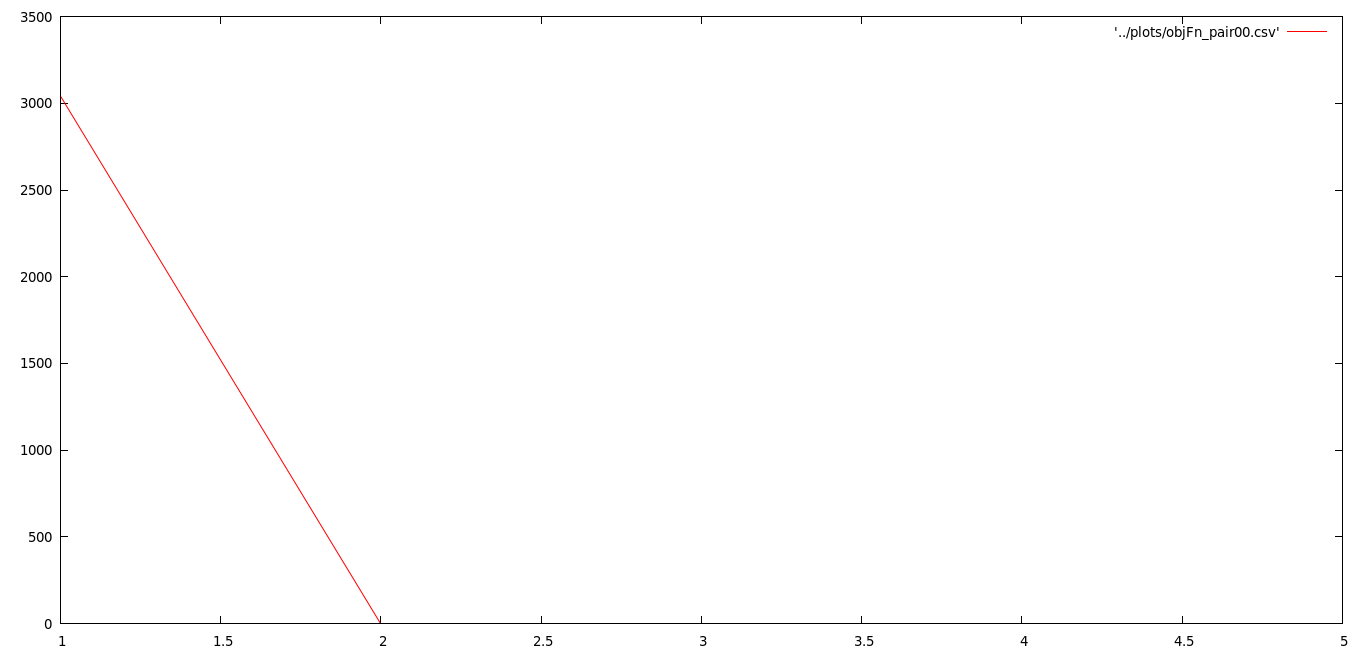
\includegraphics[scale=0.35]{objFn_pair00}}

\subsection{Estimating synthetic transformations} 
As the next step, we `synthesize' transformed pointclouds (by translating and rotating one of the pointclouds by known quantites). For example, the transformation matrix
$$T = \begin{pmatrix}
 0.500001 & -0.866025 & 0 & 2.5 \\
 0.866025 & 0.500001 & 0 & 0 \\
        0 & 0 & 1 & 0 \\
        0 & 0 & 0 & 1
\end{pmatrix}$$
on the pointcloud \textit{pair00.pcd} yields the two pointclouds (one white and one green) as shown: \\ \\
\centerline{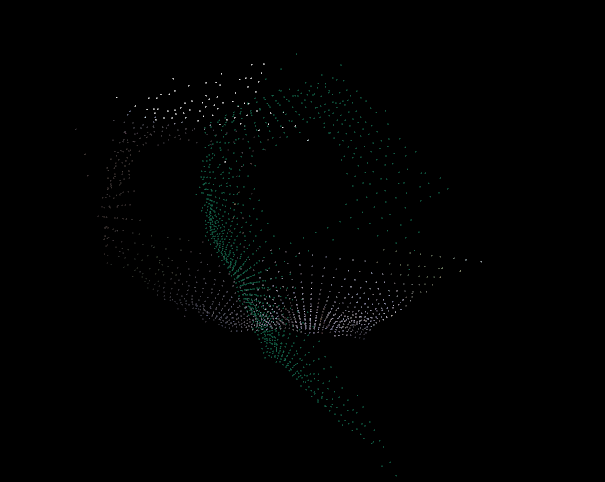
\includegraphics[scale=0.5]{synthPair}} \\ \\
We then run the matching algorithm on these pointclouds and compare the output to the (known) transformation matrix. For this particular example, the estimated transformation after five iterations is
$$T = \begin{pmatrix}
 0.60301 & -0.797733 & 0 & 2.256 \\
 0.797733 & 0.60301 & 0 & 0 \\
        0 & 0 & 1 & 0 \\
        0 & 0 & 0 & 1
\end{pmatrix}$$
which is close enough to the original value. A plot of the objective function with iteration number is shown below: \\ \\
\centerline{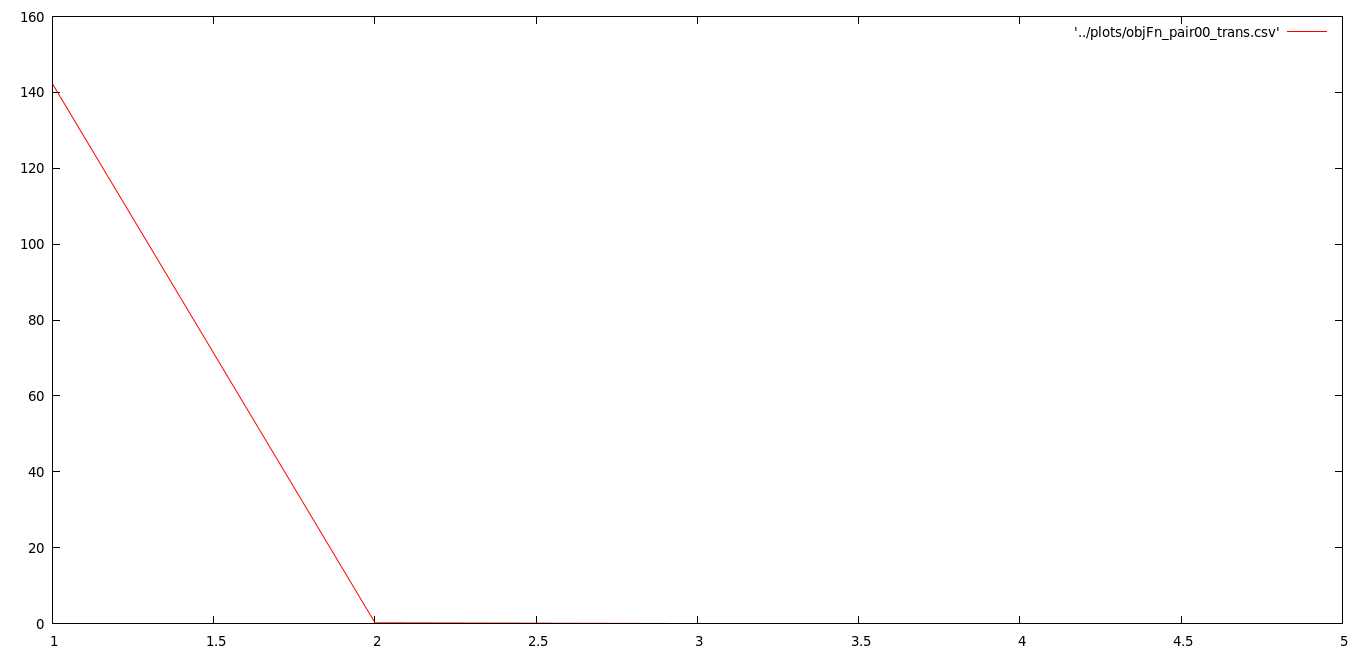
\includegraphics[scale=0.35]{objFn_pair00_trans}} \\ \\

\subsection{Estimating non-identity transformations}
Now we try to estimate the transformation between different pointclouds. Here we have significant convergence problems if the transformation is not initialised sufficiently close to the actual transformation. We think this is because the pointclouds used have relatively little overlap, and this is not sufficient to make the algorithm converge to the actual transformation. We do not include the results since we do not think this part is complete.

\section{Other Methods}
We also tried an implementation of Coherent Point Drift, see \cite{cpd} and \cite{wiki}, which we did not get time to debug and test. This is in a non-working state right now.

\section{Concluding Remarks}
We showed the algorithm working for the identity transformation and transformations that don't differ much from identity. The objective function is bounded below by zero, and almost always (at least in the synthetic transformation case) drops down to zero by the first five iterations. This shows that the solution obtained is (almost) optimal. We did not explore the parameter space (changing Gaussian variance and step size) much. However, estimation of small transformations is useful enough since two pointclouds which are captured in succession are related by transformations that are not very different from each other.

\begin{thebibliography}{9}

\bibitem{main}
  Bing Jian and Vemuri, B.C.,
  \emph{Robust Point Set Registration Using Gaussian Mixture Models}.
  IEEE Transactions on Pattern Analysis and Machine Intelligence,
  2010.
  
\bibitem{mainPre}
  Pre-print of the above paper \href{http://code.google.com/p/gmmreg/downloads/detail?name=gmmreg_PAMI_preprint.pdf}{here}.
  
\bibitem{quatParam}
  George Terzakis, Phil Culverhouse \textit{et al},
  \emph{A Recipe on the Parameterization of Rotation Matrices for Non-Linear Optimization using Quaternions}.
  Technical Report of the School of Marine Science and Engineering, Plymouth University,
  2012.
  
\bibitem{cppStuff}
  Documentation for the OpenCV, Point Cloud and Eigen libraries in C++ \href{http://docs.opencv.org/}{here},\href{http://pointclouds.org/documentation/}{here} and \href{http://eigen.tuxfamily.org/dox/}{here} respectively

\bibitem{cpd}
  Andriy Myronenko and Xubo Song,
  \emph{Point Set Registration: Coherent Point Drift}.
  IEEE Transactions on Pattern Analysis and Machine Intelligence,
  2010.

\bibitem{wiki}
  The Wikipedia article on Point Set Registration \href{http://en.wikipedia.org/wiki/Point_set_registration}{here}.

\end{thebibliography}

\end{document}